\section{Perturbing test problems (working title)} \label{app:TestProblemsPerturbed}

Since it is necessary to provide an initial guess for the control $\vec{w}$ to start the optimization routine, as detailed in Section \ref{sec:Method_Solver}, one method of validation is to perturb the exact solution for $\vec{w}$ and use this as an initial guess in the optimization solver. In the first iteration, this results in a different solution for $\rho$ and $\adj$ than the exact solution. The optimization method  converges to the exact solution, which is the/an optimal solution. We consider Test Problem 2 (maybe tag this) in Appendix \ref{app:TestProblems}, which is an exact solution for Problem \eqref{AdvDiff}, with boundary conditions \eqref{NoFlux}, and $\gamma = 0$. 
The following two perturbation functions are considered. The first perturbation is in time only and is defined as:
\begin{align*}
g(t) &= \frac{1}{2} f(t-t_0, a) \times f(t-t_0, -a)\\
&= \frac{1}{2} \frac{e^{-a/(t-t_0)}}{e^{-a/(t-t_0)} + e^{-a/(1-t -t_0)}} \times \frac{e^{a/(t-t_0)}}{e^{a/(t-t_0)} + e^{a/(1-t - t_0)}}.
\end{align*}
The normalised version is then 
\begin{align*}
\tilde g(t) = \frac{g(t)}{\max{|{g(t)}|}},
\end{align*}
so that $\max{\tilde g(t)} =1$.
A similar perturbation can be done in space, taking into account the difference in length of spatial and time domain:
\begin{align*}
h(x) &= \frac{1}{2} f(x-x_0, 2a) \times f(x-x_0, -2a)\\
&= \frac{1}{2} \frac{e^{-2a/(x-x_0)}}{e^{-2a/(x-x_0)} + e^{-2a/(1-x-x_0)}} \times \frac{e^{2a/(x-x_0)}}{e^{2a/(x-x_0)} + e^{2a/(1-x-x_0)}}.
\end{align*}
Again, the normalised version is:
\begin{align*}
\tilde h(x) = \frac{h(x)}{\max{|{h(x)}|}}.
\end{align*}
These perturbation functions are chosen such that the perturbation is smooth and respects the initial condition for $\rho$ as well as the final time condition for $\adj$, by not changing the first or final time point, see Figure \ref{Fig:PerturbationFunctions}.
The considered perturbations are applied to the exact control $\vec{w}_{ex}$ as follows:
\begin{align*}
\vec{w}_{pert1} &= \vec{w}_{ex}(1+ \epsilon \tilde g(t))\\
\vec{w}_{pert2} &= \vec{w}_{ex}(1+ \epsilon \tilde g(t) \tilde h(x)),
\end{align*}
where $a = 0.7$, $x_0 = t_0 = -0.01$ and $\epsilon = 0.1$ or $\epsilon = 0.5$.
The chosen number of points is $N =40$ and $n=41$, the ODE tolerances are $10^{-8}$ and Optimization tolerance is $10^{-4}$. The mixing rate for the optimization solver is $\lambda = 0.01$.
The results presented in Table \ref{TabApp2} show the initial error in $\vec{w}$, and the final errors in $\vec{w}$, $\rho$ and $\adj$, measured in the norm presented in Section \ref{sec:Method_Solver}, with respect to the exact solution. It can be seen that most of the errors are within the optimization tolerance, such as most final errors for $\vec{w}$ and $\rho$. Since in the optimization routine $\adj$ is obtained using the final values of $\vec{w}$ and $\rho$ it can be observed that the error in $\adj$ is generally higher than for the other two variables. Overall, these results show that the method works reliably.

\begin{figure}[h]
	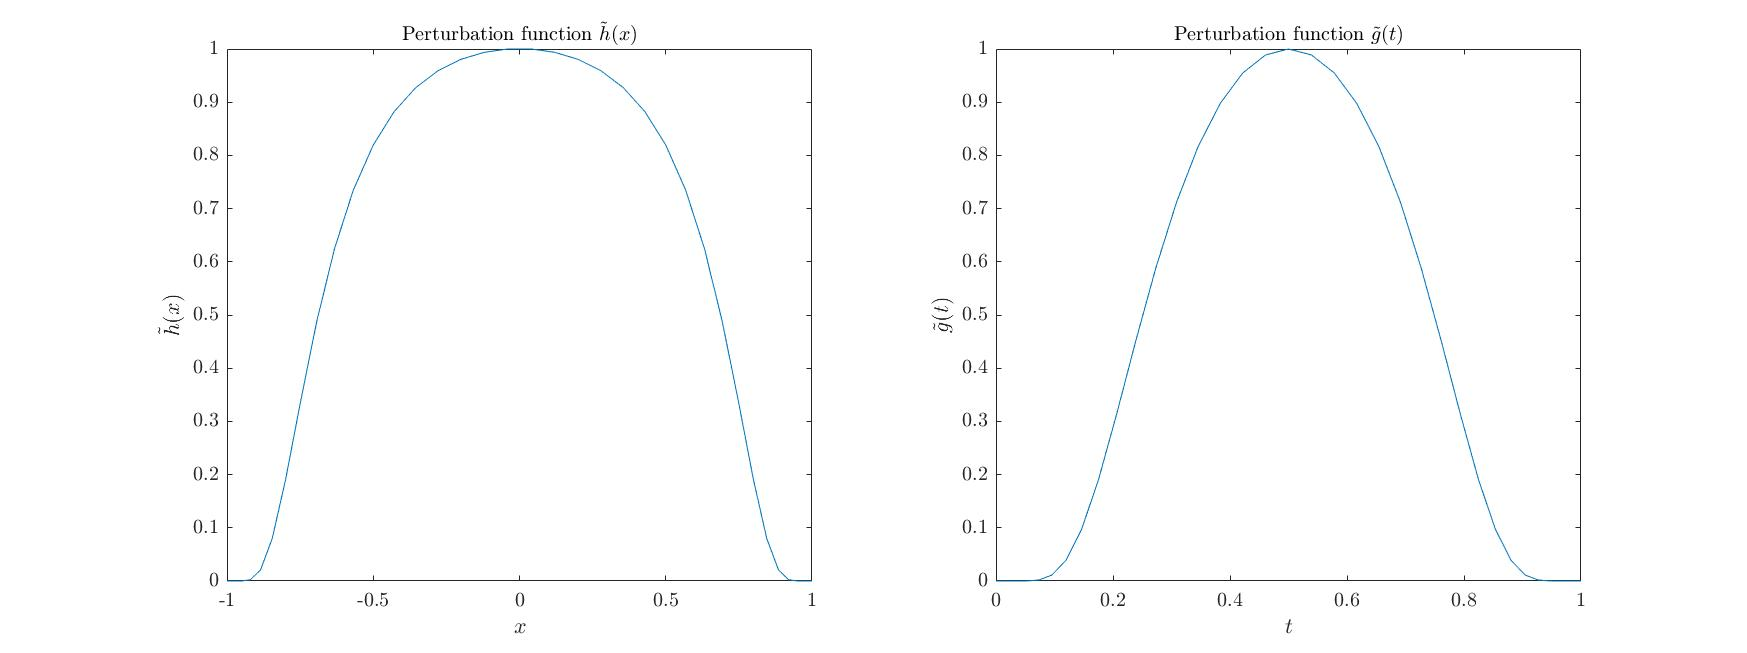
\includegraphics[scale=0.25]{PerturbationFunctions.jpg}
	\caption{Perturbation functions $\tilde h(x)$ and  $\tilde g(t)$}
	\label{Fig:PerturbationFunctions}
\end{figure} 
\begin{table}
	\begin{tabular}{ ||c |c || c || c |c | c ||}
		\hline
		                    &	& Initial Error  & Final & Error &  \\ 
		                	& $\beta$  & $\vec{w}$  & $\vec{w}$  & $\rho$ & $\adj$ \\ 
		\hline
			                & $10^{-3}$	& $0.1$  & $6.3190 \times 10^{-5}$ & $1.1648 \times 10^{-5}$ & $2.8425 \times 10^{-5}$  \\
		 $0.1\tilde g(t)$   & $10^{-1}$	& $0.1$  & $6.1449 \times 10^{-5}$ & $7.9587 \times 10^{-5}$ & $2.8405 \times 10^{-4}$ \\
		                 	& $10^{1}$	& $0.1$  & $6.1304 \times 10^{-5}$ & $7.9576 \times 10^{-5}$ & $5.8824 \times 10^{-4}$ \\
		\hline 
			                & $10^{-3}$	& $0.5$  & $2.7263 \times 10^{-4}$  & $2.9182 \times 10^{-5}$ & $3.2882 \times 10^{-5}$ \\
		$0.5 \tilde g(t)$   & $10^{-1}$	& $0.5$  & $2.7064 \times 10^{-4}$ & $2.7098 \times 10^{-4}$ &  $3.2894 \times 10^{-4}$\\
		                    & $10^{1}$	& $0.5$  & $2.7079 \times 10^{-4}$ & $2.7096 \times 10^{-4}$ & $6.8139 \times 10^{-4}$ \\
		\hline 
			                & $10^{-3}$	& $0.0855$ & $6.1809 \times 10^{-5}$ & $1.1842 \times 10^{-5}$ & $2.7355 \times 10^{-5}$ \\
		$0.1\tilde h(x)$    & $10^{-1}$	& $0.0855$ & $6.0187 \times 10^{-5}$ & $8.0212 \times 10^{-5}$ & $2.7321 \times 10^{-4}$ \\
		                    & $10^{1}$	& $0.0855$ & $6.0047 \times 10^{-5}$ & $8.0200 \times 10^{-5}$ & $5.7592 \times 10^{-4}$ \\
		\hline 
			                & $10^{-3}$	& $0.4276$  & $2.5041 \times 10^{-4}$ & $2.7429 \times 10^{-5}$ & $3.1303 \times 10^{-5}$ \\
		$0.5\tilde h(x)$    & $10^{-1}$	& $0.4276$  & $2.4833 \times 10^{-4}$ & $2.5436 \times 10^{-4}$ & $3.1332 \times 10^{-4}$ \\
	                     	& $10^{1}$	& $0.4276$  & $2.4846 \times 10^{-4}$ & $2.5435 \times 10^{-4}$ & $6.4922 \times 10^{-4}$ \\
		\hline 
    \end{tabular}
	\caption{}
\label{TabApp2}
\end{table}
